%!TEX root = ../Thesis.tex
\chapter{Unreal Engine 4}

\section{Waarom de Unreal Engine 4}

Tijdens het kiezen van een Engine waren er drie rand voorwaarden namelijk 
\begin{enumerate}
	\item gratis voor educatie, of goedkoop genoeg voor DPI om aan te schaffen
	\item Oculus en GearVR ondersteuning
	\item Een \gls{vr} systeem
\end{enumerate}

De volgende Engine’s zijn naar gekeken 
\begin{itemize}
\item Unity
\item CRYENGINE
\item Unreal Engine 4
\end{itemize}

\subsection{Unity}

\subsubsection{Licentie}
Unity heeft een educatie licentie waaronder het grootste gedeelte van de engine gratis gebruikt kan worden maar rekening houdend met de interesses van DPI, en eventuele vervolg projecten die zei willen ondernemen, zal de licentie minimaal 75€ per maand worden met daar de koste van Android builds bij.

\subsubsection{Oculus en GearVR ondersteuning}
Van de drie engine’s heeft unity de meest uitgebreide platform support. Daarnaast is Unity vaak een van de eerste keuze’s om nieuwe technieken mee te implementeren. De reden achter deze keuze is het gemak waarop plugins gemaakt kunnen worden en de voordelige / gratis pricing van Unity wat het een populaire keuze maakt voor experimenteren.

\subsubsection{Virtual Scripting}
Unity heeft zelf niet een ingebouwd \gls{vs} systeem maar via een aantal plugins kan dit wel worden toegevoegd. Deze plugins zitten wel vast aan de limitaties van een Unity Plugin. Daarnaast word dit niet officieel gesupporterd door Untiy zelf.

\subsubsection{Gebruiks gemak}
Op gebruiksgemak, in serieuze projecten, fidelity en performance loopt Unity ver achter op de \gls{ue4} en CryEngine. Onderhoudbaar en uitbreidbaarheid van Unity is meestal rampzalig door de manier waarop code voor Unity geschreven word. Vaak is Unity daarom ook niet de keuze voor grote games van hoge kwaliteit. 

Het programmeren word namelijk in een component style in c-sharp gedaan. Het programmeren in c-sharp is voor veel mensen fijn omdat dit vaak een bekende taal is. Maar het component systeem en de manier waarop Unity relatie’s afhandelt zorgt dat er extreem snel spaghetti code ontstaat. 

\subsection{CRYENGINE}
\subsubsection{Licentie}
De CRYENGINE licentie bestaat uit een “Pay what you want” model. Daarnaast beid Crytek een “CRYENGINE Insider Membership“ aan voor 50€ of 150€. 

\subsubsection{Oculus en GearVR ondersteuning}
Op het moment van schrijven ondersteund de CRYENGINE wel de Oculus maar niet de GearVR. Android ondersteuning is mogelijk maar niet officieel ondersteund door Crytek. Dit zal het lastig maken om GearVR te ondersteunen.

\subsubsection{Visual Scripting}
De CRYENGINE heeft een ingebouwd \gls{vs} systeem genaamd Flow. Dit systeem heeft helaas geen ondersteuning voor overerving en de koppeling met c++ bestaat alleen uit het maken van nieuwe nodes en het aanspreken van graphs in c++.

\subsubsection{Gebruiksgemak}
De CryEngine staat bekend als een moeilijke Engine om in te beginnen maar heeft ondertussen bewezen een goede keuze te zijn voor game ontwikkelaars en grotere teams.

Door het gebrek aan persoonlijke ervaring kan ik hier minder over zeggen. Maar door het gebrek aan GearVR ondersteuning is er hier niet meer in verdiept.

\subsection{Unreal Engine 4}
\subsubsection{Licentie}
Het gebruik van de \gls{ue4} is compleet gratis voor educatie en niet-game applicaties zoals architectuur, visualisatie, films etc. Dit betekend dat zowel tijdens het afstuderen als mogelijke vervolg projecten van DPI er geen licentie kosten betaald hoeven te worden.

\subsubsection{Oculus en GearVR ondersteuning}
\gls{ue4} ondersteund zowel de Oculus als Gear VR. Daarnaast ondersteund het ook de meeste randapparatuur voor \gls{vr} zoals Leap Motion en Kinect. Updates hiervoor komen vaak wel later dan voor Unity.
\subsubsection{Visual Scripting}
Unreal heeft een uitgebreid \gls{vs} systeem wat nauw samenwerkt met c++. Alle functies die in c++ beschikbaar zijn zijn beschikbaar via Blueprints. Van elke Blueprint kan ook direct de source code ingesprongen worden, zelfs voor de functies uit de \gls{ue4} libraries.

Het koppelen van c++ aan Blueprints is vrij simpel en ondersteund ook het creëren van events in c++ en functionaliteit hieraan via Blueprints te koppelen.

\subsubsection{Gebruiks gemak}
De leer curve van \gls{ue4} is redelijk stijl maar binnen een paar weken is het mogelijk de belangrijkste te leren. Een punt om rekening mee te houden is dat het zomaar iets maken in de \gls{ue4} vaak verkeerd uitpakt. Daarom is het belangrijk de documentatie, van het onderdeel waar je mee bezig bent, goed te lezen.

Als de basis principes eenmaal onder de knie zijn kan er extreem snel ontwikkeld, en geprototyped, worden met de \gls{ue4} door de implementatie van \gls{vs} en een strakke en goed uitgedachte UI.

\subsubsection{Conclusie}
De CRYENGINE valt af vanwege zijn gebrek aan GearVR support. Dan blijft de keuze over tussen Unity en \gls{ue4}. Untiy heeft een minder style learning curve maar geavanceerde 3D technieken zullen uiteindelijk toch geleerd moeten worden om een hoge kwaliteit te behalen. 

Het visuele scripting systeem van Unity is beperkt en mist de kracht en flexibiliteit die nodig is om deze scriptie succesvol af te ronden. Daar in tegen beid het visuele scripting systeem van \gls{ue4} wel deze mogelijkheden.

\section{Blueprints}
Blueprints is het visuele scripting systeem van \gls{ue4} en wat deze scriptie mogelijk maakt. De beschrijving van Unreal zelf is als volgt:

“Blueprints are special assets that provide an intuitive, node-based interface that can be used to create new types of Actors and script level events; giving designers and gameplay programmers the tools to quickly create and iterate gameplay from within Unreal Editor without ever needing to write a line of code.”

Blueprints ziet er als volgt uit:

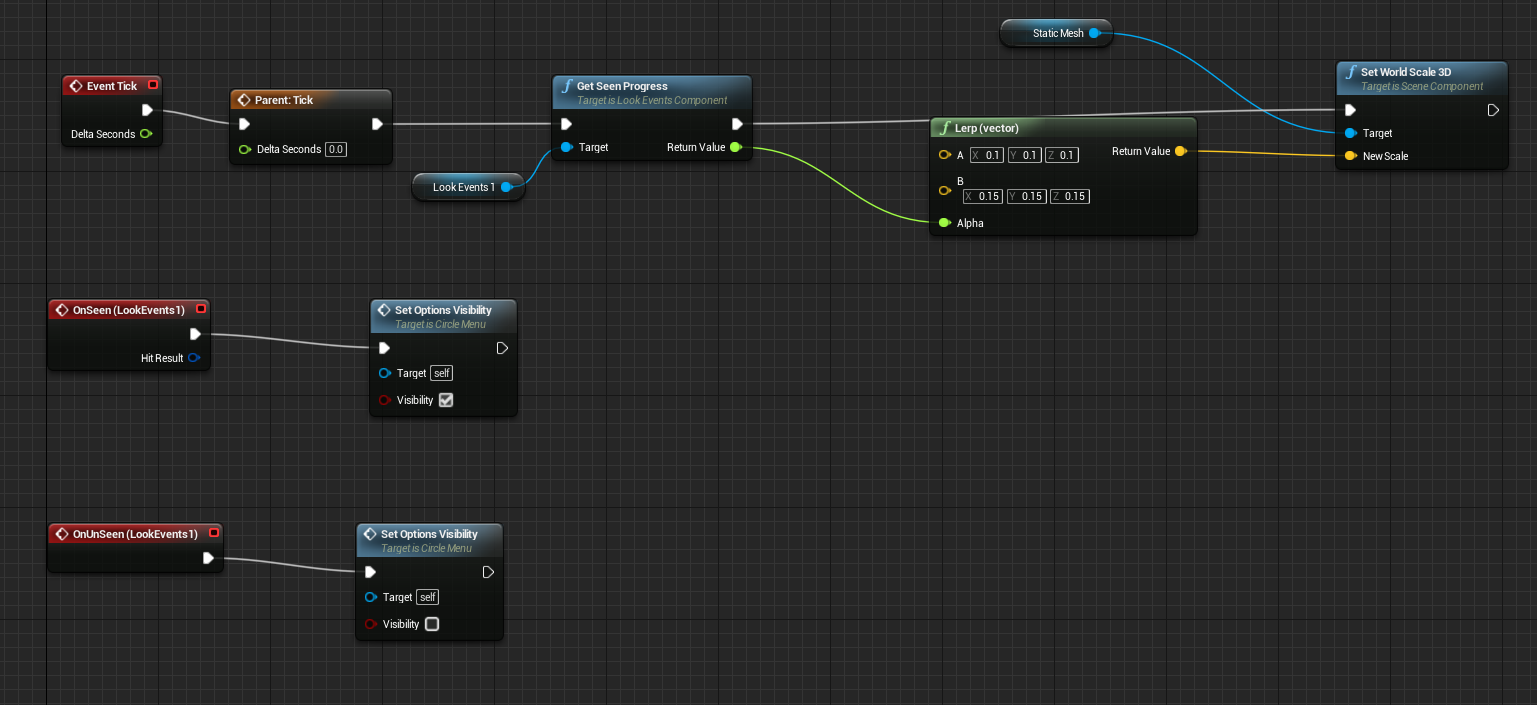
\includegraphics{BluePrintSeenExample}

Een hele kort samenvatting zou zijn dat de rode nodes Events zijn en dus aangeven wanneer iets gebeurd, de witte lijnen bepalen de volgorde waarin de nodes worden uitgevoerd, de blauwe nodes zijn functies en de rest zijn variabelen of pure transformatie van data.